% -----------------------------------------------------------------------------
\section{Data Model Examples}
\label{sec:examples}
% -----------------------------------------------------------------------------

%\subsection{LacI/TetR Toggle Switch}

This section illustrates how to use the SBOL data model by specifying the design of a LacI/TetR toggle switch similar to those constructed in \cite{Gardner2000}. This design is visualized conceptually in \ref{images:toggle} and in detail in \ref{images:toggleswitch_modular}. 

Conceptually, the toggle switch is constructed from two mutually repressing genes.  
With repressors LacI and TetR, this results in a bi-stable system that will tend to settle into a state where precisely one of the two repressors is strongly expressed, repressing the other.
Each of these repressors can have its activity disrupted by a small molecule (IPTG for LacI, aTc for TetR), which enables the system to be ``toggled'' from one state to the other by dosing it with the appropriate small molecule.

\twotwozero{
\begin{figure}[ht]
\begin{center}
\includegraphics[width=0.33\textwidth]{images/toggle-highlevel2.pdf}
\caption[]{Conceptual diagram of LacI/TetR toggle switch: the LacI 
  and TetR transcription factors are arranged to mutually repress each other's expression, 
  creating a bi-stable system.  Transition between the two states
  is triggered by the small-molecule signals aTc (which disrupts TetR
  repression) and IPTG (which disrupts LacI repression).}
\label{images:toggle}
\end{center}
\end{figure}

\begin{figure}[ht]
\begin{center}
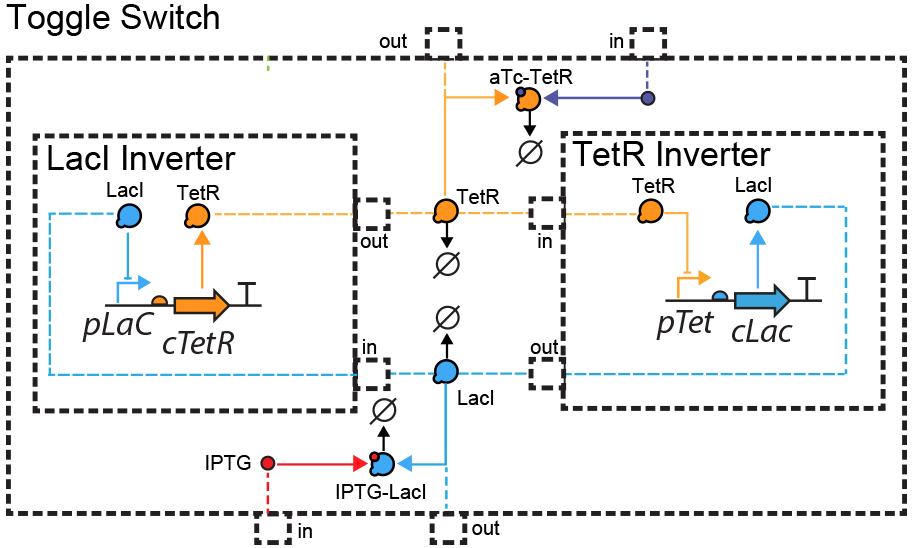
\includegraphics[width=\textwidth]{images/toggleswitch_modular2}
\caption[]{Design of a LacI/TetR toggle switch. This design is composed of two inverter sub-designs, each containing a single gene. These genes mutually repress each other's expression via their encoded protein transcription factors, LacI and TetR. Furthermore, both LacI and TetR are bound by specific small molecules that sequester them and prevent them from acting as repressors. In this design, arrows represent different molecular interactions, including the repression of pLac via LacI, the non-covalent binding of IPTG to LacI, the transcription of TetR mRNA, and the translation of TetR. Dashed lines serve to map between transcription factors in the inverter sub-designs and those in the overall toggle switch design.}
\label{images:toggleswitch_modular}
\end{center}
\end{figure}
}

The LacI/TetR toggle switch is modeled in SBOL as two parallel hierarchies of structure and function. The structural hierarchy of the toggle switch is represented using \sbol{ComponentDefinition}s:
\begin{itemize}
\item The base elements of the hierarchy are DNA components, transcription factor proteins, and small molecules. As an example, \ref{uml:ex_comp_defs} is a UML diagram of the \sbol{ComponentDefinition} objects that represent these elements.
\item Base elements are composed to form more complex structures at the top of the hierarchy, including genes and non-covalent complexes between transcription factor proteins and small molecules. As an example, \ref{uml:ex_comp_def_compo} is a UML diagram of the composite \sbol{ComponentDefinition} objects that represent the TetR gene and IPTG-LacI complex.
\end{itemize}

\begin{figure}[ht]
\begin{center}
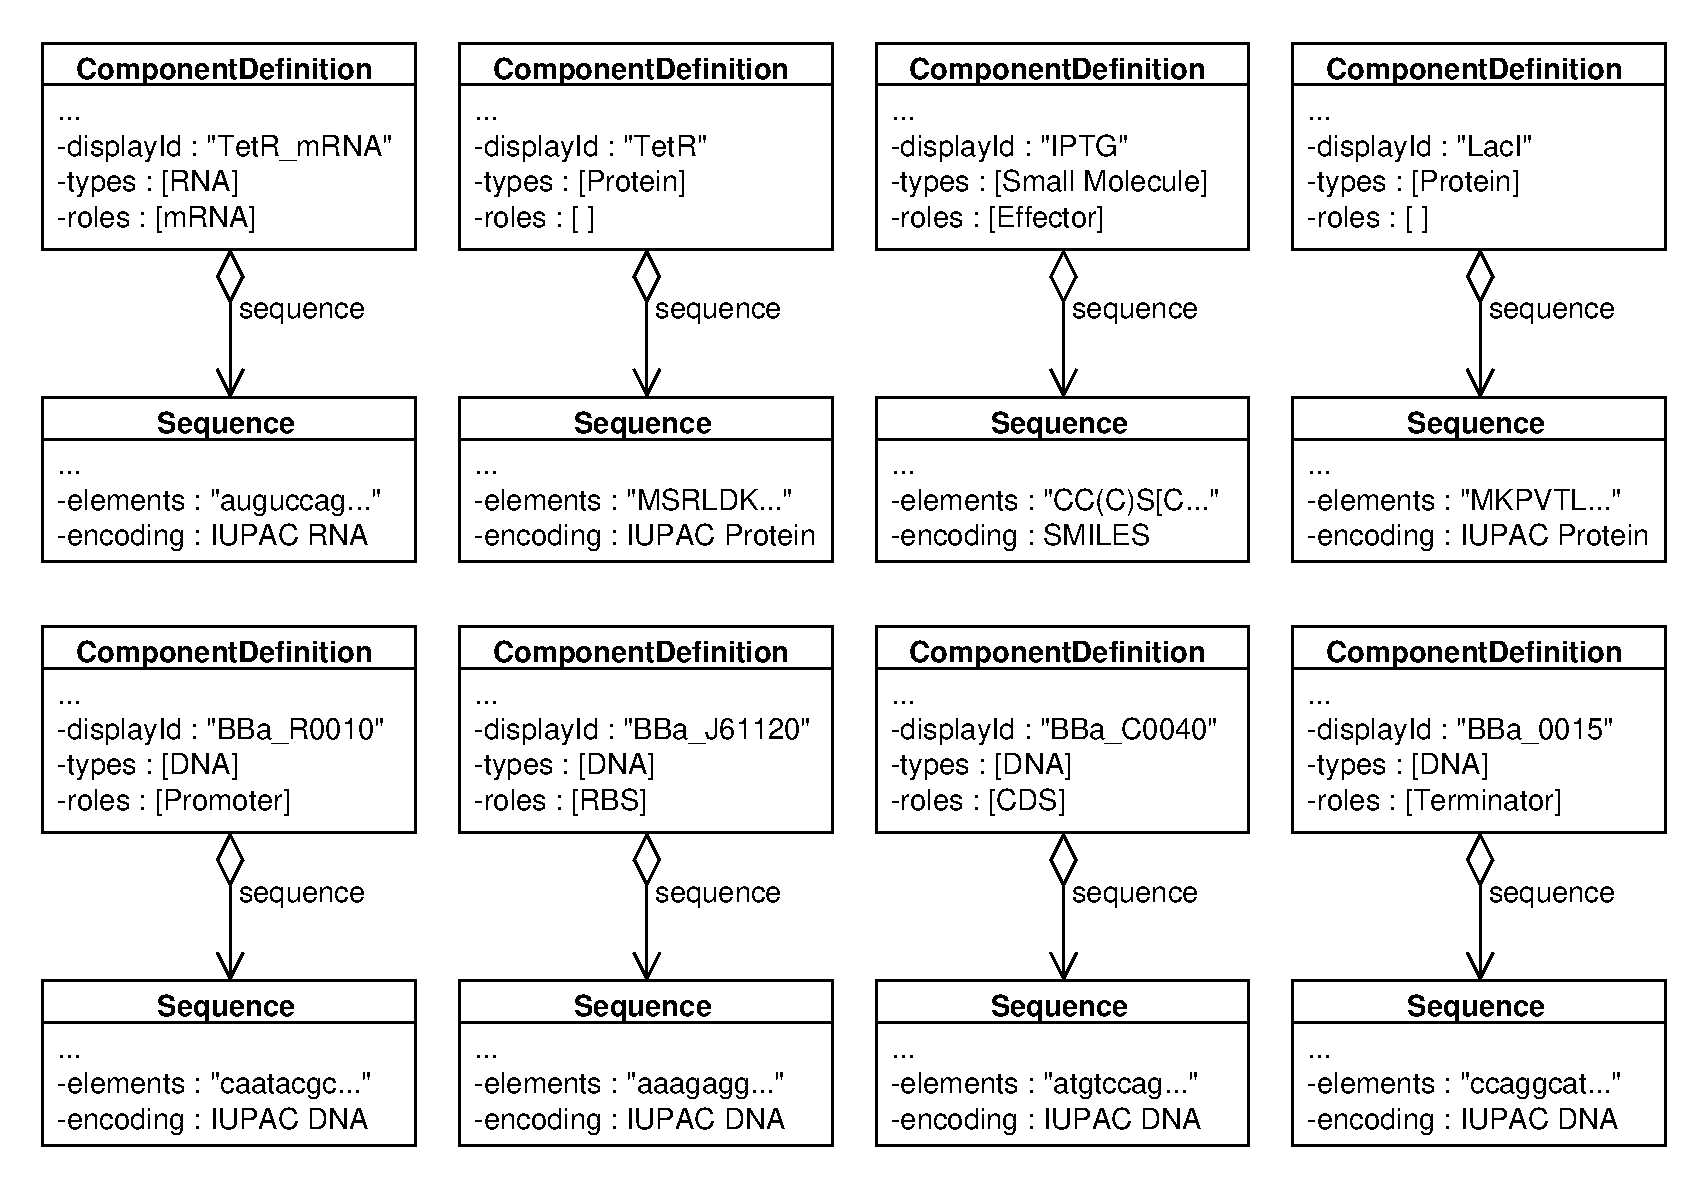
\includegraphics[width=\textwidth]{example_uml/toggle_1}
\caption[]{\sbol{ComponentDefinition} objects for the LacI inverter. These include \sbol{ComponentDefinition} objects based on DNA parts from the iGEM Parts Registry and  \sbol{ComponentDefinition} objects that represent TetR mRNA, TetR, LacI, and IPTG. Each \sbol{ComponentDefinition} is associated with a \sbol{Sequence} that has an \external{IUPAC DNA/RNA} or \external{IUPAC protein} \sbol{encoding}, except the \sbol{ComponentDefinition} of IPTG, which is associated with a \sbol{Sequence} that has a \external{SMILES} \sbol{encoding}.}
\label{uml:ex_comp_defs}
\end{center}
\end{figure}


\begin{figure}[ht]
\begin{center}
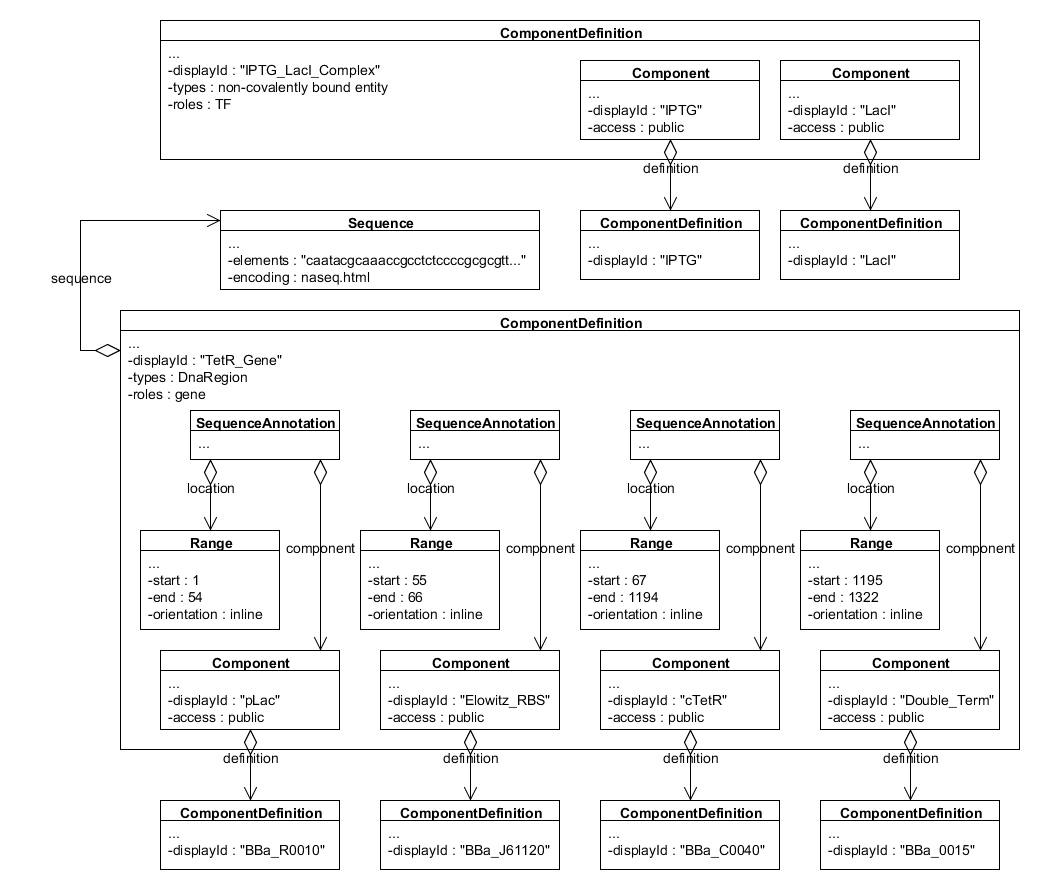
\includegraphics[width=\textwidth]{example_uml/toggle_2}
\caption[]{Composite \sbol{ComponentDefinition} objects for the LacI inverter. In the case of the \sbol{ComponentDefinition} that represents the TetR gene, its sub-\sbol{Component} objects are located as \sbol{Range}s along its \sbol{Sequence} using \sbol{SequenceAnnotation} objects. The \sbol{ComponentDefinition} that represents the IPTG-LacI complex, however, has no \sbol{Sequence} and its sub-\sbol{Component} objects are composed without any data about their relative positions.}
\label{uml:ex_comp_def_compo}
\end{center}
\end{figure}


The functional hierarchy of the toggle switch is represented using
\sbol{ModuleDefinition}s:
\begin{itemize}
\item The base elements of the hierarchy are LacI-dependent repression of TetR expression (the LacI inverter) and TetR-dependent repression of LacI (the TetR inverter). As an example, \ref{uml:ex_mod_def} is a UML diagram of the \sbol{ModuleDefinition} that represents the LacI inverter.
\item Base elements are composed to form the toggle switch at the top of the hierarchy.  As an example, \ref{uml:ex_mod_def_compo} is a UML diagram of the \sbol{ModuleDefinition} that represents the toggle switch.
\end{itemize}

\begin{figure}[ht]
\begin{center}
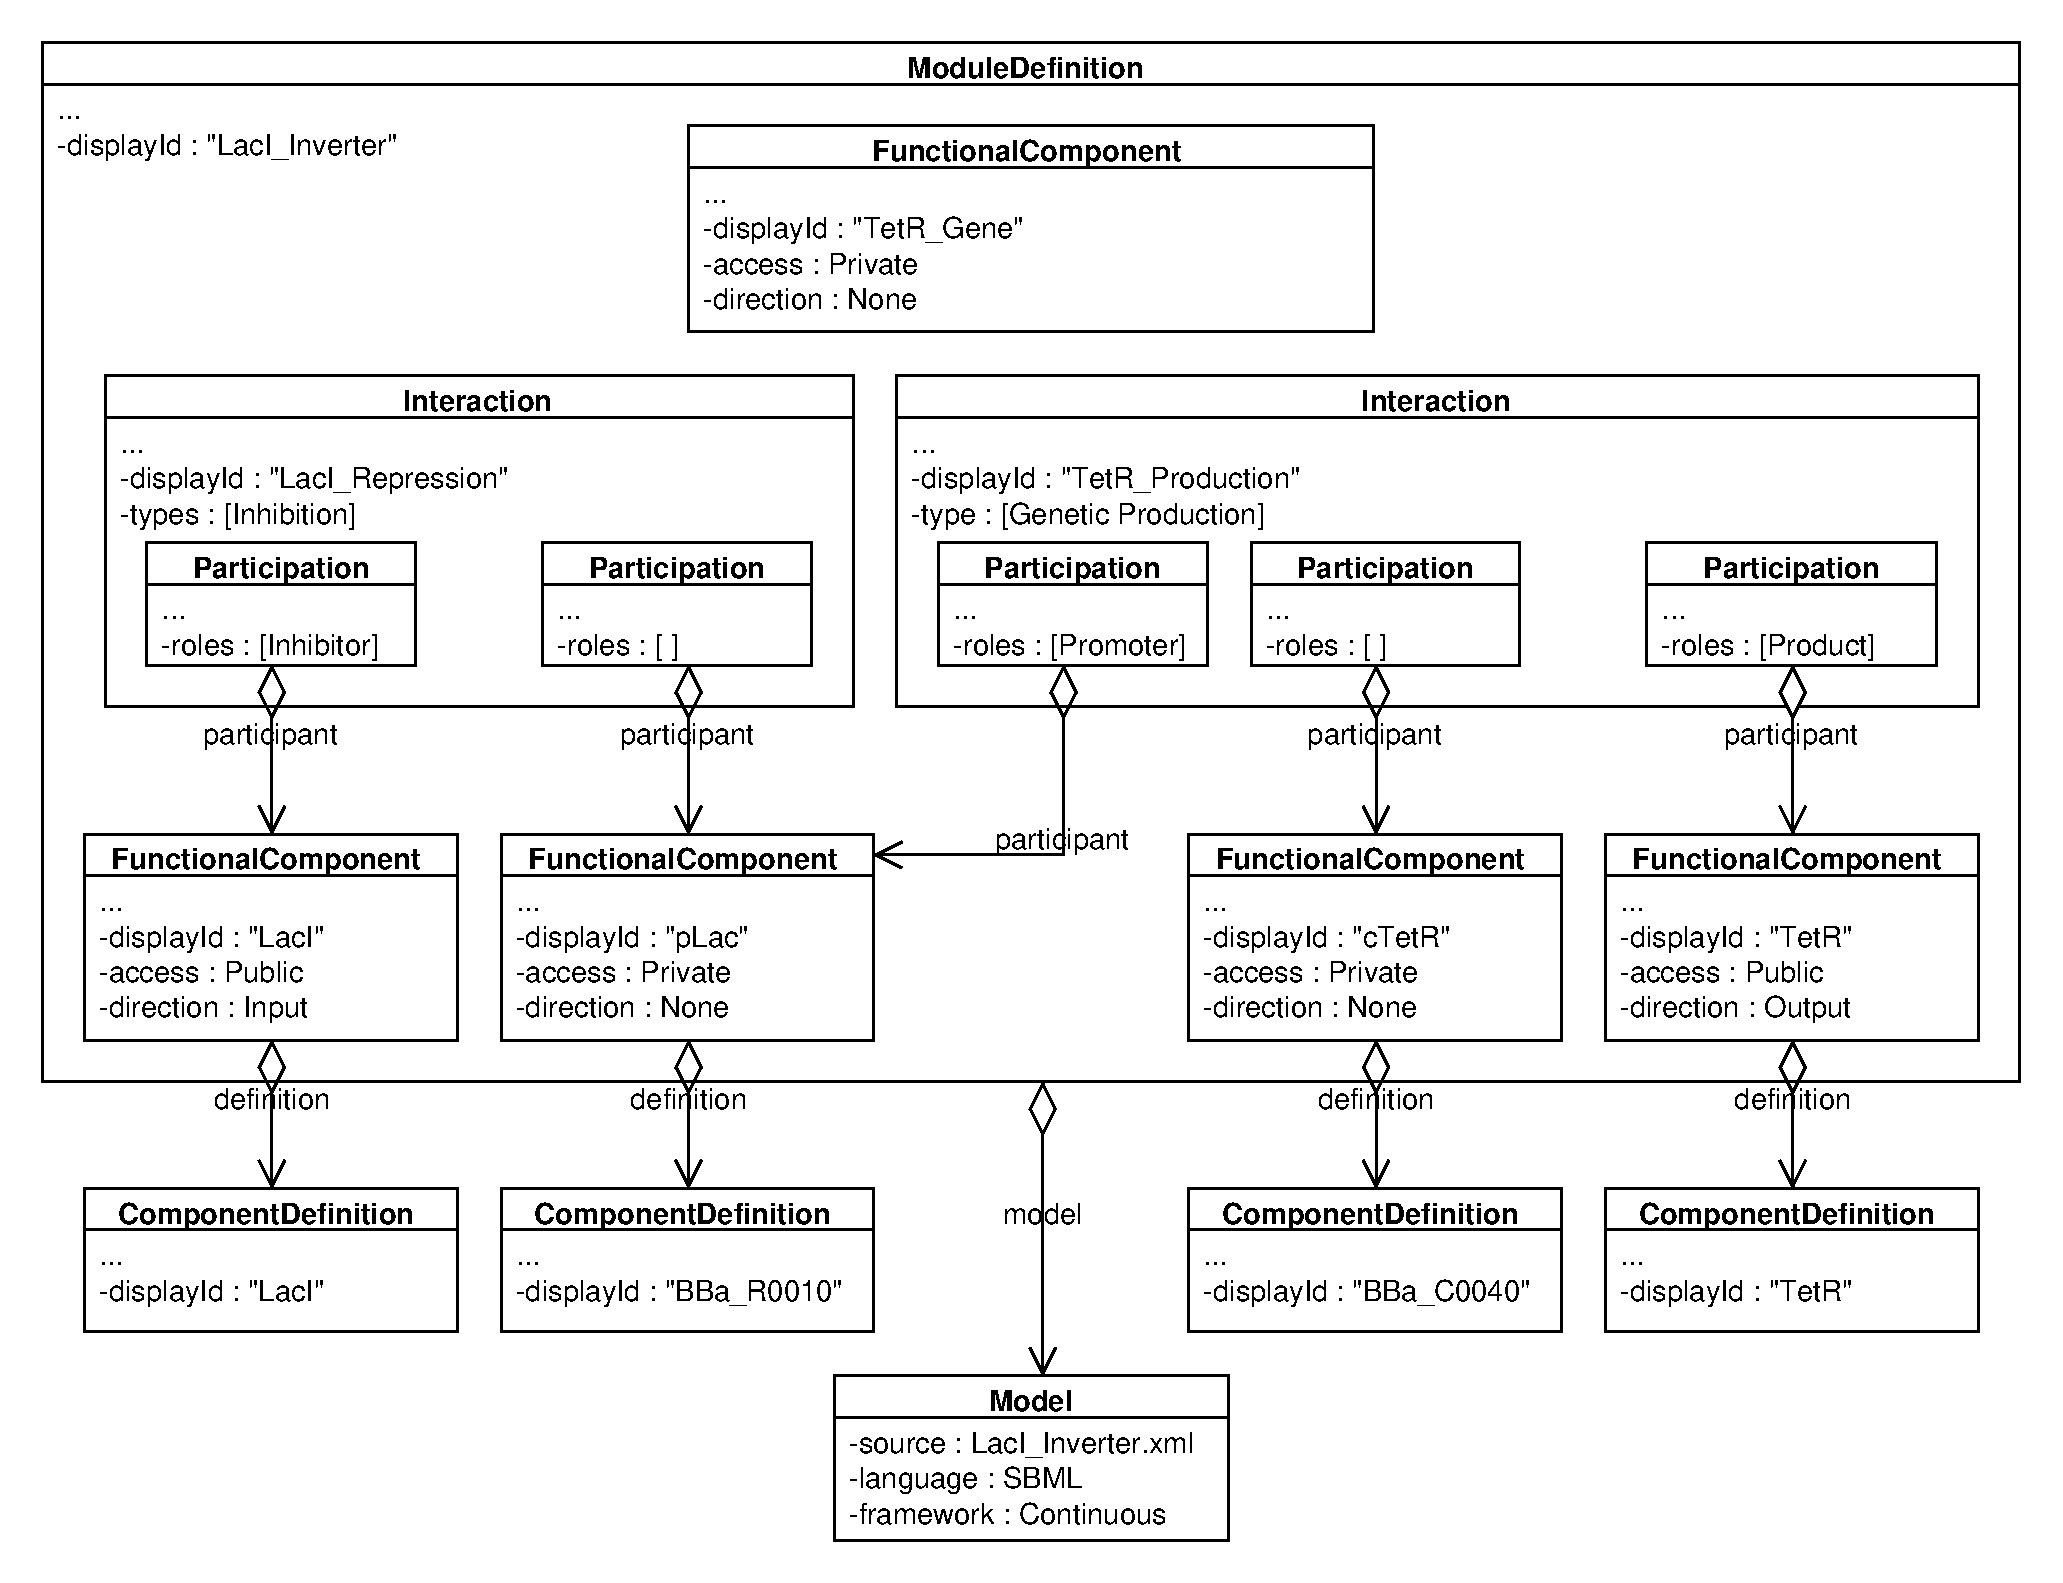
\includegraphics[width=\textwidth]{example_uml/toggle_3}
\caption[]{\sbol{ModuleDefinition} of the LacI inverter. This \sbol{ModuleDefinition} contains \sbol{FunctionalComponent} objects that instantiate the \sbol{ComponentDefinition} objects for the LacI/TetR transcription factors and TetR gene. These \sbol{FunctionalComponent} objects participate in a repression \sbol{Interaction} and a genetic production \sbol{Interaction}, thereby indicating which biological structures carry out the function of the LacI inverter \sbol{ModuleDefinition}. In this case, the transcription and translation of TetR are represented as a single genetic production \sbol{Interaction} that abstracts away the presence of the intermediate TetR mRNA.  In addition, this \sbol{ModuleDefinition} is also associated with a continuous \sbol{Model} written in the SBML source file ``LacI\_Inverter.xml.''}
\label{uml:ex_mod_def}
\end{center}
\end{figure}

\begin{figure}[ht]
\begin{center}
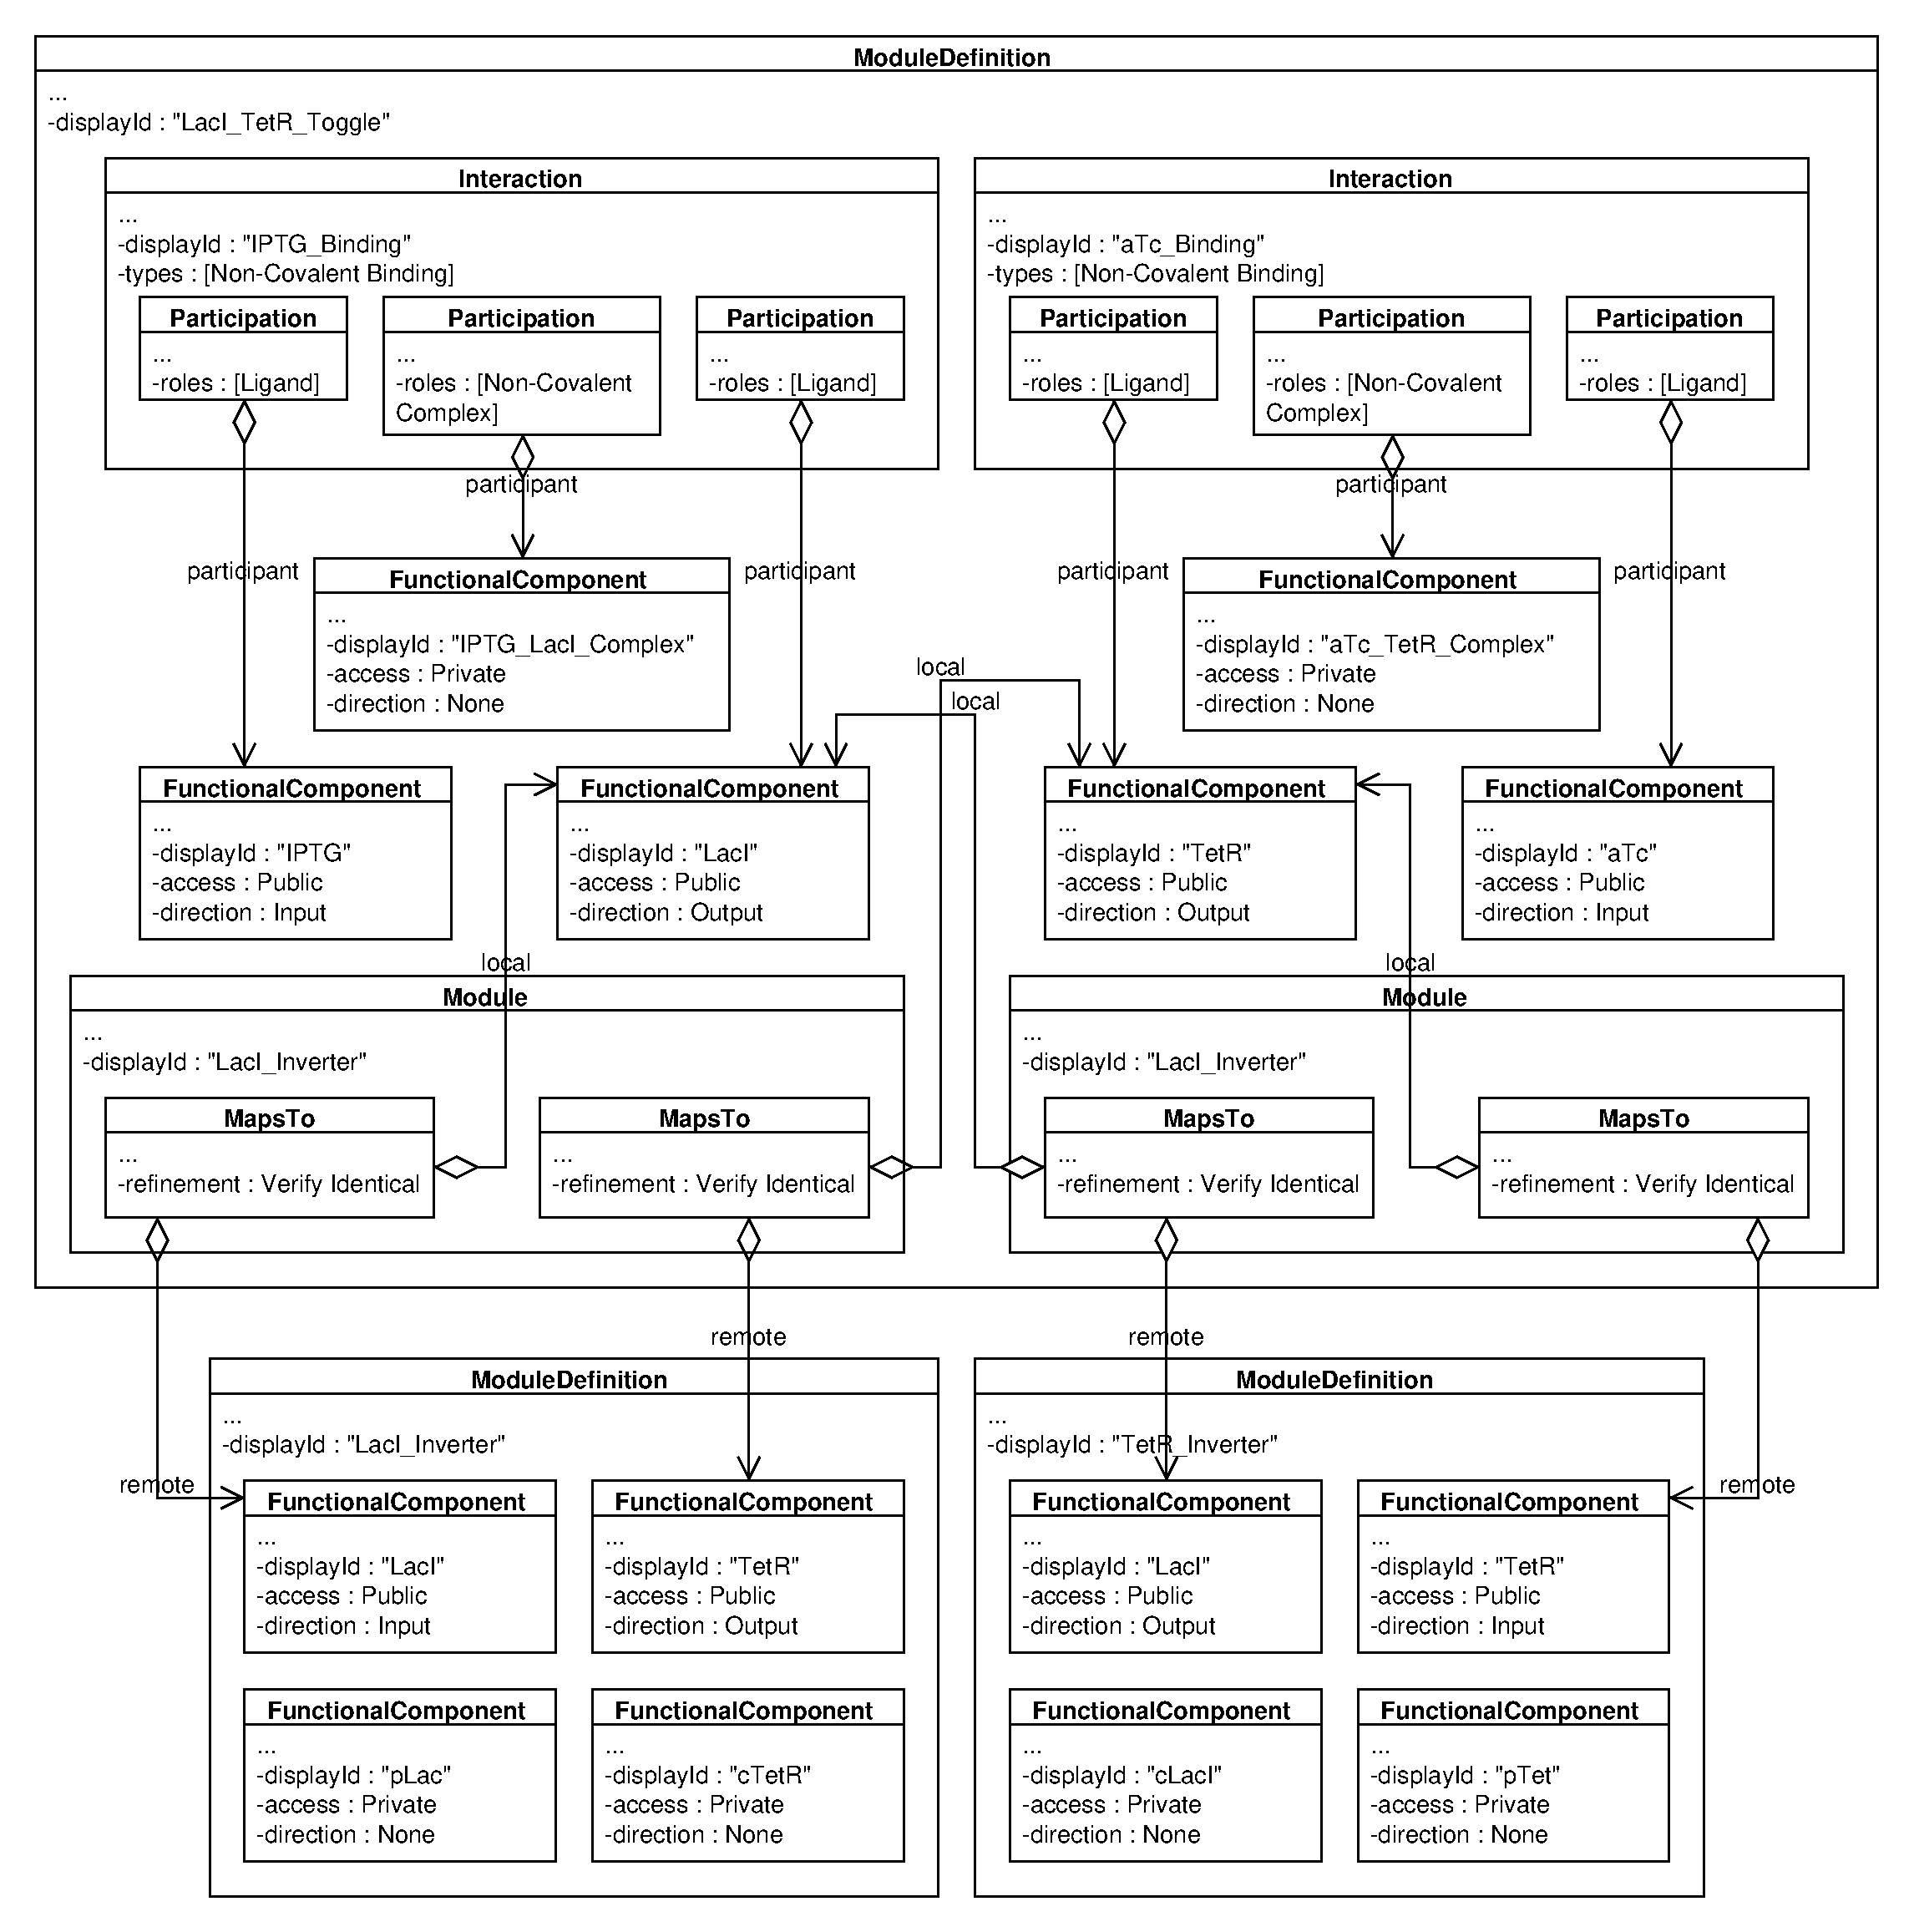
\includegraphics[width=\textwidth]{example_uml/toggle_4}
\caption[]{Composite \sbol{ModuleDefinition} of the LacI/TetR toggle switch. This \sbol{ModuleDefinition} contains the \sbol{Module} objects that instantiate LacI and TetR inverter \sbol{ModuleDefinition} objects. It also contains \sbol{FunctionalComponent} objects that instantiate the \sbol{ComponentDefinition} objects for the LacI/TetR transcription factors and IPTG/aTc small molecules. These \sbol{FunctionalComponent} objects each participate in a non-covalent binding \sbol{Interaction}. To complete the composition of the toggle switch, \sbol{MapsTo} objects are used to indicate that the output of the LacI inverter \sbol{ModuleDefinition} is identical to the input of the TetR inverter \sbol{ModuleDefinition} and vice versa.
}
\label{uml:ex_mod_def_compo}
\end{center}
\end{figure}


% Each \sbol{ModuleDefinition} also contains the \sbol{FunctionalComponent}s that participate in \sbol{Interaction}s and are defined by the same \sbol{ComponentDefinition}s as the parallel \sbol{Component}s in the structural hierarchy of the toggle switch. Finally, \sbol{MapsTo} entities are used to refine which \sbol{FunctionalComponent}s of the functional hierarchy are identical or map them to \sbol{Component}s in the structural hierarchy.

%  The first use case is to indicate with greater fidelity how a module describes the function of a composite component, namely by asserting that particular component instantiations within the module correspond to particular component instantiations within the component. 

% As an example of this use case, one might compose the structure and function of the LacI-repressible gene of the genetic toggle switch. In this example, the LacI-repressible gene and two of its subcomponents, the pLac promoter and cTetR CDS, are to be composed with the LacI inverter module. In order to compose these components with the LacI inverter module and indicate that it describes their behavior, they are instantiated inside the module. In addition, port maps are placed on the instantiation of the LacI-repressible gene to connect between its pLac plus cTetR subcomponent instantiations and the corresponding component instantiations in the module. Doing so makes it clear which subcomponent instantiations in the gene are being described by which component instantiations in the module. In this way, GDA tools for sequence editing and biochemical modeling can guarantee that their users are handling corresponding elements of a given genetic design, while GDA tools for genetic technology mapping can make explicit connections between the structural and functional elements of a design.
